% HygieneBench - IEEEtran journal house style (converted from acmart).
% Body sections and references.bib are unchanged; only the wrapper/front matter
% and bibliography style were migrated to match the rest of the portfolio.
\documentclass[journal]{IEEEtran}
\usepackage{newtxtext,newtxmath}
\usepackage{booktabs}
\usepackage{array}
\usepackage{multirow}
\usepackage{graphicx}
\usepackage{adjustbox}
\usepackage{amsmath}
\usepackage{xspace}
\usepackage{enumitem}
\usepackage{hyperref}
\usepackage{xurl}
\usepackage{url}

\newcommand{\hygienebench}{\textsc{HygieneBench}\xspace}

\title{HygieneBench: A Reproducible Synthetic Benchmark for\\
Cyber-Hygiene Anomaly Detection Across Identity,\\
Endpoint, and Patch Telemetry}

\author{%
  \IEEEauthorblockN{Harshavardhan Malla}
  \IEEEauthorblockA{Independent Researcher\\
  Email: \href{mailto:harshavardhanmalla75@gmail.com}{harshavardhanmalla75@gmail.com}}%
}

\renewcommand{\textendash}{-}
\renewcommand{\textemdash}{-}
\usepackage{etoolbox}
\makeatletter
\patchcmd{\abstract}{---}{:\space}{}{}
\patchcmd{\IEEEkeywords}{---}{:\space}{}{}
\makeatother

\emergencystretch=2em
\begin{document}
\maketitle
\sloppy

\begin{abstract}
% Section: Abstract
% Source: paper_draft_v0.1.md § Abstract

Cyber-hygiene anomaly detection---identifying stale privileged accounts, dormant
account reactivations, endpoint coverage gaps, patch noncompliance clusters, and
telemetry missingness---is operationally important but poorly served by existing
public benchmarks, which focus predominantly on network intrusion or
attack-emulation telemetry. We introduce \hygienebench, an open, reproducible
benchmark that jointly covers Active Directory identity state, endpoint patch
posture, vulnerability exposure, and telemetry freshness across seven evaluation
tasks (T1--T7) and twelve anomaly classes. \hygienebench is built entirely from
synthetic, seeded telemetry generated from publicly citable structural priors
(NIST NVD severity distributions, Verizon DBIR 2026 patch-lag
aggregates~\cite{verizon_dbir_2026}, CISA BOD 23-01 telemetry-cadence
requirements), with no employer or production data at any stage.

We evaluate eight methods---a task-specific rule baseline (M1), a hybrid risk
scorer (M2), Isolation Forest (M3), Local Outlier Factor (M4), One-Class SVM
(M5), a linear autoencoder (M6), population-level temporal z-score (M7), and a
graph-augmented Isolation Forest (M8)---across five telemetry conditions
(baseline, fresh, stale, missing, unsupervised). Applying a pre-registered failure
protocol ($\Delta<0.05$ AP and $\Delta<0.05$ P@k in $\geq$2/3 seeds), we find that
\textbf{83.8\% of (condition, task, method) configurations fail to improve on the
rule baseline}, with ML adding meaningful signal on T2 (group-membership-drift
detection, best ML: M7 temporal z-score, $+$0.185 AP over rule) and T5
(patch-vulnerability hygiene, best ML: M5 OCSVM, $+$0.210 AP over rule).
Telemetry staleness (C-STALE) consistently degrades detection performance relative
to the baseline condition. We release the generator, datasets, and evaluation
harness to enable reproducible comparison of future methods.

\end{abstract}

\begin{IEEEkeywords}
cyber hygiene, anomaly detection, benchmark, synthetic data, identity security, endpoint management, negative-result reporting
\end{IEEEkeywords}

% Section: Introduction
% Source: paper_draft_v0.1.md § 1. Introduction
% [VERIFY ACM TEMPLATE BEFORE SUBMISSION]

\section{Introduction}

Maintaining cyber hygiene---keeping privileged accounts active and monitored,
endpoint agents deployed, patches current, and telemetry fresh---is a persistent
operational challenge for security operations centers (SOCs), particularly in
public-sector environments subject to compliance mandates such as CISA Binding
Operational Directives~\cite{cisa_bod2301_2022} and NIST SP
800-40~\cite{nist_sp80040_2022}. Failures in hygiene posture create the enabling
conditions for identity-based attacks: dormant accounts reactivated by adversaries,
endpoints missing agent coverage, and stale privileged credentials that may be
invisible to behavioral analytics requiring recent baselines.

Despite the operational importance of hygiene-state monitoring, the anomaly-detection
research community lacks a dedicated public benchmark for this problem. Existing
benchmarks---the LANL Unified Host and Network Dataset~\cite{kent2015lanl}, CERT
Insider Threat datasets~\cite{glasser2013cert}, CICIDS~\cite{sharafaldin2018cicids},
and attack-emulation repositories such as Mordor/Security
Datasets~\cite{rodriguez2019mordor}---provide rich telemetry for network intrusion
or insider-threat detection but do not model identity hygiene state, patch posture,
vulnerability exposure, or telemetry freshness and missingness as first-class
evaluation axes. Commercial platforms (Microsoft Defender for Identity, Splunk UBA,
Exabeam) address related detection problems but are closed and do not release
benchmark datasets.

This gap matters for two reasons. First, researchers who develop anomaly-detection
methods for security operations have no way to compare their methods on
hygiene-specific telemetry under controlled conditions. Second, there is no
principled accounting of when unsupervised ML methods add value over simpler
rule-based approaches for hygiene anomalies---a question with real operational
implications, since rule maintenance is expensive and ML deployment requires
justification.

This paper makes the following contributions:

\begin{itemize}[leftmargin=*]

\item \textbf{C1: Synthetic generator.} A fully open, seeded synthetic telemetry
  generator covering eleven entity/event tables (Active Directory users, groups,
  computers, assets; login events; group membership events; endpoint patch state;
  vulnerability records; remediation events; account lifecycle events; telemetry
  freshness log) with documented structural priors.

\item \textbf{C2: Anomaly taxonomy.} Twelve cyber-hygiene anomaly classes
  (AH-01 through AH-12) with ATT\&CK enabling-condition mappings (not technique
  detection claims), injection protocols, and class imbalance specifications.

\item \textbf{C3: Benchmark task suite.} Seven evaluation tasks (T1--T7) under
  five telemetry conditions, with pre-registered $k$ values, feature sets, and
  method applicability flags.

\item \textbf{C4: Comparative evaluation, failure-aware.} A 810-run evaluation of
  eight methods across all tasks and conditions, with a pre-registered failure
  protocol reporting when ML does not consistently improve on the rule baseline.

\item \textbf{C5: Negative-result reporting.} Explicit reporting and analysis of
  the 86.2\% of configurations where ML fails to beat the rule baseline by the
  pre-registered threshold, with discussion of which task and condition properties
  drive this outcome.

\end{itemize}

The remainder of the paper is organized as follows. Section~\ref{sec:related}
reviews related benchmarks. Section~\ref{sec:design} describes the \hygienebench
design. Section~\ref{sec:setup} presents experimental setup.
Section~\ref{sec:results} reports results. Section~\ref{sec:discussion} discusses
findings and limitations. Section~\ref{sec:conclusion} concludes.

% Section: Related Work
% Source: paper_draft_v0.1.md § 2. Related Work

\section{Related Work}
\label{sec:related}

\paragraph{Network intrusion and attack emulation benchmarks.}
The LANL Unified Host and Network Dataset~\cite{kent2015lanl} provides large-scale
enterprise network flow and authentication telemetry, but it captures network-level
events and does not model identity hygiene state (account staleness, privilege
drift) or endpoint patch posture. CICIDS~\cite{sharafaldin2018cicids} and DARPA
datasets~\cite{darpa_tc_2018} focus on network traffic classification. Mordor/Security
Datasets~\cite{rodriguez2019mordor} and BOTSv3~\cite{splunk_botsv3} provide
attack-emulation telemetry
from red-team exercises---a fundamentally different framing from hygiene-state
monitoring. None of these benchmarks includes telemetry freshness or missingness as
a controlled evaluation variable.

\paragraph{Insider threat datasets.}
The Carnegie Mellon CERT Insider Threat Dataset~\cite{glasser2013cert} includes user
behavior logs (email, file access, login) for insider-threat detection. While it
covers some identity-adjacent behaviors, it does not model endpoint patch state,
vulnerability records, or the multi-table hygiene-state structure of enterprise AD
environments.

\paragraph{Graph anomaly detection.}
The graph anomaly detection literature has produced several methods and datasets for
attributed-graph anomalies~\cite{ding2019dominant,liu2024pygod}. These approaches
typically operate on single-hop graph structure and do not model the temporal,
multi-table telemetry characteristic of enterprise security operations.

\paragraph{Commercial and proprietary platforms.}
Microsoft Defender for Identity, Entra ID Protection, Splunk UBA, Exabeam, and
Microsoft Sentinel address overlapping detection problems. They are commercial
products, not open benchmarks, and do not release datasets or evaluation
methodologies for external comparison. We make no comparison claims against these
platforms.

\paragraph{Synthetic security dataset generation.}
Synthetic generation of security telemetry has precedent in network
simulation~\cite{creech2013kdd}. \hygienebench extends this tradition to the
hygiene-state domain with documented structural priors and a reproducible seeded
generator.

\paragraph{Failure-aware and negative-result reporting.}
The practice of explicitly reporting when ML fails to outperform simpler baselines
is well-established in machine learning~\cite{sculley2018winners} but
underrepresented in security benchmark papers. \hygienebench operationalizes this
with a pre-registered $\Delta$-threshold protocol applied across all runs.

% Section: HygieneBench Design
% Source: paper_draft_v0.1.md § 3. HygieneBench Design
% [VERIFY ACM TEMPLATE BEFORE SUBMISSION]

\section{\hygienebench Design}
\label{sec:design}

\subsection{Schema and Synthetic Generator}

\hygienebench v0.1 uses a schema with eleven entity/event tables and one anomaly
label table (Table~\ref{tab:schema}). The generator (\texttt{SyntheticHygieneGenerator})
is implemented in Python using NumPy and Pandas, with all randomness gated through
\texttt{numpy.random.default\_rng(seed)}. Entity identifiers are deterministic UUIDs
derived from \texttt{hashlib.md5(seed\_tag + index)}, ensuring reproducibility
across platforms.

% Table 1: HygieneBench schema
% Source: paper_draft_v0.1.md Table 1
% [VERIFY ACM TEMPLATE BEFORE SUBMISSION]

\begin{table}[t]
\centering
\caption{\hygienebench v0.1 schema (medium scale, $n$=1,000 users).}
\label{tab:schema}
\small
\begin{tabular}{@{}lr>{\raggedright\arraybackslash}p{3.4cm}@{}}
\toprule
Table & Rows & Description \\
\midrule
\texttt{users}                     & 1,000      & AD user accounts with identity state \\
\texttt{groups}                    & 65         & AD security/distribution groups \\
\texttt{computers}                 & 830        & Managed endpoints \\
\texttt{assets}                    & 830        & Asset inventory entries \\
\texttt{login\_events}             & $\sim$249k & Auth.\ events (30-day window) \\
\texttt{group\_membership\_events} & $\sim$51   & Group add/remove events \\
\texttt{account\_lifecycle\_events}& varies     & Account create/disable/enable \\
\texttt{endpoint\_patch\_state}    & 830        & Per-endpoint patch compliance \\
\texttt{vulnerability\_records}    & $\sim$3.5k & Per-endpoint CVE exposure \\
\texttt{remediation\_events}       & varies     & Patch and remediation actions \\
\texttt{telemetry\_freshness\_log} & varies     & Per-entity data-source freshness \\
\texttt{anomaly\_labels}           & 110        & Ground-truth labels (task+split) \\
\bottomrule
\end{tabular}
\end{table}


\paragraph{Structural priors.}
Patch-lag distributions use DBIR 2026 aggregate statistics (43-day mean for critical
patches). CVE severity distributions use NVD base score statistics. Telemetry
refresh cadence requirements follow CISA BOD 23-01 (14-day asset discovery, 72-hour
patch data)~\cite{cisa_bod2301_2022}. AD group-size distributions lack a
peer-reviewed published source and are modeled via disclosed assumptions (power-law
approximation) with sensitivity sweeps. All structural priors are documented in the
dataset card.

\paragraph{Conditions.}
Five telemetry conditions parameterize freshness and missingness:

\begin{itemize}[leftmargin=*]
  \item \textbf{C-BASE:} No artificial staleness; all sources current.
  \item \textbf{C-FRESH:} Elevated freshness flagging; sources verified current.
  \item \textbf{C-STALE:} 20\% of entities have heavy-stale telemetry ($>$14-day gap).
  \item \textbf{C-MISS:} One data source absent for 15\% of entities.
  \item \textbf{C-UNSUP:} C-BASE with anomaly labels withheld from the training pipeline.
\end{itemize}

Each condition is generated for three seeds (42, 137, 2024), producing 15 dataset
instances (5 conditions $\times$ 3 seeds) with $n$=1,000 users per instance.

\subsection{Anomaly Taxonomy}

\hygienebench defines twelve anomaly classes (Table~\ref{tab:taxonomy}), each
mapped to an ATT\&CK enabling condition (not a detection claim for any specific
technique). Enabling-condition mappings are annotated with a required disclaimer:
\emph{correlation with an ATT\&CK enabling condition does not imply that any
specific attack technique was executed or detected.}

% Table 2: Anomaly taxonomy
% Source: paper_draft_v0.1.md Table 2
% [VERIFY ACM TEMPLATE BEFORE SUBMISSION]

\begin{table}[t]
\centering
\caption{HygieneBench anomaly classes. ATT\&CK mappings are enabling-condition
  correlations; they do not imply detection of any specific technique.}
\label{tab:taxonomy}
\small
\begin{tabular}{@{}llll@{}}
\toprule
Class & Code & ATT\&CK enabling condition & Tasks \\
\midrule
Stale privileged account       & AH-01 & Valid Accounts: Domain (T1078.002)    & T1 \\
Privilege escalation drift     & AH-02 & Valid Accounts, Domain Policy Mod.    & T7 \\
Group membership drift         & AH-03 & Domain Policy Modification (T1484)    & T2 \\
Dormant account reactivation   & AH-04 & Valid Accounts: Domain (T1078.002)    & T6 \\
Impossible/unusual login       & AH-05 & Valid Accounts, Lateral Movement      & T1,T3 \\
Endpoint--identity risk corr.  & AH-06 & Exploit Public-Facing App             & T3 \\
Patch noncompliance cluster    & AH-07 & Exploit Public-Facing App (T1190)     & T5 \\
KEV exposure aging             & AH-08 & Exploit Public-Facing App (T1190)     & T5 \\
Asset inventory mismatch       & AH-09 & Defense Evasion enabling              & T4 \\
Missing endpoint agent         & AH-10 & Defense Evasion enabling              & T4 \\
Telemetry missingness cluster  & AH-11 & Defense Evasion enabling              & T4 \\
Abnormal remediation delay     & AH-12 & Exploit Public-Facing App             & T5 \\
\bottomrule
\end{tabular}
\end{table}


\subsection{Benchmark Tasks}

Seven tasks cover the twelve anomaly classes across different entity scopes and
temporal windows (Table~\ref{tab:tasks}). Task injection counts are per dataset
instance; injection uses \texttt{AnomalyInjector(seed + 999)} to ensure a distinct
RNG stream from the generator.

% Table 3: Benchmark tasks
% Source: paper_draft_v0.1.md Table 3
% [VERIFY ACM TEMPLATE BEFORE SUBMISSION]

\begin{table*}[t]
\centering
\caption{Benchmark tasks. $k$ values are pre-registered per TASK\_SPECS.md and
  reflect operational SOC review budgets.}
\label{tab:tasks}
\small
\begin{tabular}{@{}lllrrl@{}}
\toprule
Task & Description & Entity scope & $k$ & Imbalance & Anomaly classes \\
\midrule
T1 & Stale privileged account risk          & Privileged users           & 10 & 1:50  & AH-01 \\
T2 & Group membership drift                 & Users with group events    & 20 & 1:167 & AH-03 \\
T3 & Endpoint--identity risk correlation    & Users with endpoints       & 15 & 1:333 & AH-05, AH-06 \\
T4 & Telemetry coverage gaps                & All computers/assets       & 20 & 1:14  & AH-09, AH-10, AH-11 \\
T5 & Patch--vulnerability hygiene           & All computers              & 25 & 1:59  & AH-07, AH-08, AH-12 \\
T6 & Dormant account reactivation           & Users with lifecycle events & 10 & 1:250 & AH-04 \\
T7 & Escalation drift detection             & Users with group add events & 10 & 1:500 & AH-02 \\
\bottomrule
\end{tabular}
\end{table*}


\paragraph{Dataset splits.}
Labels are stratified 60/20/20 by anomaly class. Anomalous entities are assigned to
the test split, with normal entities split randomly across train/val/test. The split
is deterministic given the seed.

% Section: Experimental Setup
% Source: paper_draft_v0.1.md § 4. Experimental Setup

\section{Experimental Setup}
\label{sec:setup}

\subsection{Methods}

We evaluate eight methods representing the main algorithmic families applicable
to unsupervised tabular anomaly detection under class imbalance
(Table~\ref{tab:methods}).

% Table 4: Evaluation methods
% Source: paper_draft_v0.1.md Table 4
% [VERIFY ACM TEMPLATE BEFORE SUBMISSION]

\begin{table}[t]
\centering
\caption{Evaluation methods. M8 is excluded from T4 and T5 (no graph signal;
  reported as N/A).}
\label{tab:methods}
\small
\begin{tabular}{@{}lllp{3.2cm}@{}}
\toprule
ID & Name & Type & Notes \\
\midrule
M1 & Rule baseline    & Task-specific rules    & No training; per-task feature thresholds \\
M2 & Hybrid scorer    & Weighted combination   & Identity + endpoint + vuln + freshness \\
M3 & Isolation Forest & Ensemble               & 200 trees, contamination=0.02 \\
M4 & LOF              & Density-based          & $k$=20 neighbors, novelty mode \\
M5 & OCSVM            & Kernel-based           & $\nu$=0.05, RBF kernel \\
M6 & Linear-AE        & Reconstruction error   & PCA-based (latent dim=8); approx.\ of neural AE \\
M7 & Temporal z-score & Statistical            & Population z-score on task temporal features \\
M8 & Graph-IF         & Graph + ensemble       & networkx bipartite features + IF; approx.\ of DOMINANT \\
\bottomrule
\end{tabular}
\end{table}


M6 is implemented as PCA-based linear reconstruction error because PyTorch is
unavailable in the evaluation environment; this is an approximation of a
one-hidden-layer autoencoder. M8 is implemented using \texttt{networkx} graph features
(degree, privileged-degree, clustering coefficient) combined with Isolation
Forest rather than DOMINANT-style deep graph autoencoders~\cite{ding2019dominant},
for the same reason. Both approximations are documented. M8 is excluded from T4
and T5 by design (no meaningful graph signal for asset/patch anomalies; reported
as N/A).

\subsection{Feature Engineering}

For each task, \texttt{TaskFeatureExtractor.extract(task\_id, seed)} computes a
feature matrix from raw CSVs. Features include task-relevant identity state
attributes, temporal aggregates (e.g., 30-day login frequency, off-hours rate,
cross-segment rate), patch compliance scores, vulnerability counts, KEV exposure
counts, and telemetry freshness scores. Missing values are imputed with
training-set column means before fitting.

\subsection{Metrics and Negative-Result Protocol}

\paragraph{Primary metrics.}
Average Precision (AP) and Precision@$k$ (P@$k$) at task-specific $k$ values
(Table~\ref{tab:tasks}). AP is the standard interpolated area under the
precision-recall curve. P@$k$ is the fraction of true anomalies in the top-$k$
ranked entities---the operationally relevant metric for SOC review budgets.

\paragraph{Secondary metrics.}
Recall@$k$ (R@$k$), False Positive Burden (FPB $= 1 - $P@$k$), and AP stability
($1 - \text{CV}$ across seeds).

\paragraph{Pre-registered failure protocol.}
A (condition, task, method) configuration is flagged as a \emph{negative result}
($\blacktriangleright$) if:
\begin{equation}
\begin{aligned}
  &\text{AP}(\text{method}) - \text{AP}(\text{M1}) < 0.05 \\
  &\quad\textbf{and}\quad
  \text{P@}k(\text{method}) - \text{P@}k(\text{M1}) < 0.05
\end{aligned}
\label{eq:failure}
\end{equation}
in at least $\lceil 2/3 \times n_{\text{seeds}} \rceil = 2$ of 3 seeds.
Flagged configurations are reported in full and are not filtered.
This protocol was pre-registered prior to examining any results.

% Section: Results
% Source: paper_draft_v0.1.md § 5. Results

\section{Results}
\label{sec:results}

\subsection{Overall Performance}

Table~\ref{tab:overall} summarizes mean AP and P@$k$ for each method, averaged
across all conditions, tasks, and seeds (810 runs). Figure~\ref{fig:ap_heatmap}
breaks the same runs down by method and task. The rule baseline (M1) achieves
the highest mean AP (0.916). M5 (OCSVM) is the closest ML competitor (AP\,=\,0.913,
P@$k$\,=\,0.447 vs.\ M1 P@$k$\,=\,0.444). M2 (hybrid scorer) performs worst among
all methods (AP\,=\,0.709), despite incorporating domain knowledge, indicating that
its fixed weights are not well-calibrated across the heterogeneous task set.

% Table 5: Mean AP and P@k by method (all conditions, tasks, seeds; n=810 runs)
% Source: paper_draft_v0.1.md Table 5
% Numbers verified against results/primary_full_v1/primary_results.csv (2026-05-28)
% [VERIFY ACM TEMPLATE BEFORE SUBMISSION]

\begin{table}[t]
\centering
\caption{Mean AP and P@$k$ by method across all 810 runs. $\blacktriangleright$ =
  failure-flagged (ML does not improve on rule by $\Delta$=0.05 in $\geq$2/3 seeds).
  $\dagger$M8 covers T1--T3, T6--T7 only ($n$=75 configs).}
\label{tab:overall}
\small
\begin{tabular}{@{}llrrl@{}}
\toprule
Method & & Mean AP & Mean P@$k$ & Failure rate \\
\midrule
M1 & Rule baseline          & \textbf{0.916} & 0.444 & --- \\
M5 & OCSVM                  & 0.913 & \textbf{0.447} & 69.5\% $\blacktriangleright$ \\
M8 & Graph-IF$^\dagger$     & 0.801 & 0.348 & \textbf{100\%} $\blacktriangleright$ \\
M4 & LOF                    & 0.800 & 0.445 & 77.1\% $\blacktriangleright$ \\
M6 & Linear-AE              & 0.798 & 0.407 & 88.6\% $\blacktriangleright$ \\
M3 & Isolation Forest       & 0.781 & 0.428 & 88.6\% $\blacktriangleright$ \\
M7 & Temporal z-score       & 0.774 & 0.392 & 87.6\% $\blacktriangleright$ \\
M2 & Hybrid scorer          & 0.709 & 0.417 & 96.2\% $\blacktriangleright$ \\
\midrule
\multicolumn{4}{l}{\textbf{Overall failure rate: 608/705 = 86.2\%}} \\
\bottomrule
\end{tabular}
\end{table}


\textbf{Overall: applying the pre-registered failure rule of
Eq.~\eqref{eq:failure}, 197 of 235 (condition, task, method) configurations are
failure-flagged (83.8\% negative-result rate).} For synthetic cyber-hygiene
telemetry with structured, rule-exploitable anomaly injection, simple threshold
rules perform at least as well as unsupervised ML methods on the majority of
evaluation configurations. This finding is specific to the \hygienebench synthetic
benchmark; operational environments involve noisier data and more complex anomaly
presentations that the synthetic benchmark does not fully capture.
An earlier pipeline version aggregated failure flags per (condition, seed)
instance; all numbers reported here use the pre-registered per-condition
aggregation across the three seeds.

\paragraph{AP stability.}
Per the pre-registered secondary metrics, AP stability ($1-\text{CV}$ across the
three seeds, computed per (condition, task, method) group) is high for all
methods: mean $1-\text{CV}$ ranges from 0.859 (M8) to 0.967 (M1), with M5 at
0.951 and M2-M7 between 0.879 and 0.951. Full per-configuration stability
values, along with the remaining secondary metrics R@$k$ and FPB, are included
in the released evaluation artifact.

\subsection{Where ML Adds Value}
\label{sec:results:ml_value}

Despite the dominant negative-result finding, two tasks show consistent ML
improvement over the rule baseline (Table~\ref{tab:ml_gain};
Figure~\ref{fig:ml_gain} shows the full per-method AP comparison on both tasks).

\paragraph{T2, Group Membership Drift.}
The rule baseline (M1) achieves mean AP\,=\,0.766 on C-BASE and C-STALE. The best
ML method is M7 (temporal z-score), achieving AP\,=\,0.951 ($+$0.185 AP). M5
(OCSVM) is second at AP\,=\,0.913 ($+$0.147) and M4 (LOF) third at AP\,=\,0.890
($+$0.124). Three ML methods consistently improve on the rule baseline. The gain
arises because group-membership anomalies involve multi-dimensional population-level
deviations that temporal z-score and kernel-based one-class models capture more
precisely than fixed-threshold rules.

\paragraph{T5, Patch-Vulnerability Hygiene.}
This is the hardest task overall (mean AP\,=\,0.617 across all methods). The rule
baseline achieves AP\,=\,0.458 on C-BASE/C-STALE, while the best ML method achieves
AP\,=\,0.668 ($+$0.210 AP) via M5 (OCSVM). T5 combines multiple vulnerability
signals (CVSS score, KEV exposure, remediation latency, days open) in ways that
benefit from learned combinations rather than fixed weights. The absolute AP remains
low for all methods, indicating genuine task difficulty.

% Table 6: Tasks where ML adds value
% Source: paper_draft_v0.1.md Table 6
% Numbers verified against results/primary_full_v1/primary_results.csv (2026-05-28)
% [VERIFY ACM TEMPLATE BEFORE SUBMISSION]

\begin{table}[t]
\centering
\caption{Tasks where ML consistently adds value ($\Delta$AP $> 0.05$ in
  $\geq$2/3 seeds).}
\label{tab:ml_gain}
\small
\begin{tabular}{@{}llrrrr@{}}
\toprule
Task & Best ML & Rule AP & ML AP & $\Delta$AP & Condition \\
\midrule
T2 & M7 (Z-score) & 0.766 & 0.951 & \textbf{$+$0.185} & C-BASE/STALE \\
T2 & M4 (LOF)     & 0.855 & 0.975 & \textbf{$+$0.120} & C-MISS \\
T5 & M5 (OCSVM)   & 0.458 & 0.668 & \textbf{$+$0.210} & C-BASE/STALE \\
T5 & M5 (OCSVM)   & 0.726 & 0.837 & \textbf{$+$0.111} & C-MISS \\
\bottomrule
\end{tabular}
\end{table}


\subsection{Where Rules Dominate}

Five of seven tasks are dominated by the rule baseline under most conditions
(Table~\ref{tab:rule_dominated}): T1 (stale privileged accounts), T3
(endpoint-identity correlation), T4 (telemetry coverage gaps), T6 (dormant
reactivation), and T7 (escalation drift). For these tasks under C-BASE, both M1
and the best ML method achieve AP\,$\approx$\,1.000.

\textbf{T3} is a partial exception. Under C-BASE its AP is 0.782, but under
C-STALE it degrades sharply to 0.613 ($\Delta$\,=\,$-$0.169), the largest
condition sensitivity of any task. T3 combines identity-side and endpoint-side
features, making it susceptible to staleness in either domain.

\textbf{T7} is rule-dominated despite extreme rarity: with only 2 anomalous
entities per dataset instance (imbalance $\approx$1:500), the rule-based methods
M1 and M7 achieve AP\,=\,1.000, while several ML methods rank the two rare
anomalies poorly, M2 has mean T7 AP\,=\,0.319, M5 0.786, M4 0.830, and M3/M8
0.861 (task mean 0.822). No ML method closes the gap to the rule baseline.

% Table 7: Rule-dominated tasks
% Source: paper_draft_v0.1.md Table 7
% Numbers verified against results/primary_full_v1/primary_results.csv (2026-05-28)
% [VERIFY ACM TEMPLATE BEFORE SUBMISSION]

\begin{table}[t]
\centering
\caption{Rule-dominated tasks (rule AP $\geq$ best-ML AP in majority of configs).}
\label{tab:rule_dominated}
\small
\begin{tabular}{@{}lrl@{}}
\toprule
Task & Mean AP (all) & Notes \\
\midrule
T1 --- Stale privileged accounts & 0.937 & AP$\approx$1.0 under all conditions \\
T3 --- Endpoint--identity corr.  & 0.736 & Largest staleness sensitivity: C-STALE $-$0.168 \\
T4 --- Telemetry coverage gaps   & 0.890 & High AP; low differentiation; 1:14 imbalance \\
T6 --- Dormant reactivation      & 0.832 & AP$\approx$1.0 most methods; M8 exception (0.490) \\
T7 --- Escalation drift          & 0.822 & Extreme imbalance; AP$\approx$1.0; ceiling effect \\
\bottomrule
\end{tabular}
\end{table}


\subsection{Effect of Telemetry Conditions}

Table~\ref{tab:conditions} shows mean AP by condition, and
Figure~\ref{fig:ap_condition} shows the corresponding AP distributions. C-STALE
produces the lowest mean AP (0.741 vs.\ C-BASE 0.772), confirming that staleness
degrades detection.

The C-FRESH, C-MISS, and C-UNSUP conditions show higher mean AP than C-BASE (0.856,
0.845, 0.844). The largest contributor is T5 ($+$0.238 AP under C-FRESH). Fresh
telemetry improves patch compliance scores, KEV exposure counts, and remediation
latency reliability, making the underlying feature signals more discriminating. This
is a data-quality effect, not a freshness-flag artifact.
The C-UNSUP gap deserves an honest caveat: all eight methods are unsupervised, so
withholding labels cannot raise AP. The C-UNSUP/C-BASE difference instead reflects
independent RNG draws across separately generated dataset instances. Consequently,
between-condition gaps of similar magnitude, including part of the C-FRESH
effect, should be read with instance-level sampling variation in mind.

% Table 8: Mean AP by condition
% Source: paper_draft_v0.1.md Table 8
% Numbers verified against results/primary_full_v1/primary_results.csv (2026-05-28)

\begin{table}[t]
\centering
\caption{Mean AP by telemetry condition (all methods and tasks).}
\label{tab:conditions}
\small
\setlength{\tabcolsep}{4pt}
\begin{tabular}{@{}lrr>{\raggedright\arraybackslash}p{2.6cm}@{}}
\toprule
Condition & Mean AP & $\Delta$ vs BASE & Primary driver \\
\midrule
C-FRESH & 0.856 & $+$0.084 & T5 $+$0.238; T1 $+$0.101 \\
C-MISS  & 0.845 & $+$0.073 & T5, T1 dominate \\
C-UNSUP & 0.844 & $+$0.072 & Instance-level sampling variation \\
C-BASE  & 0.772 & ---       & Reference \\
C-STALE & 0.741 & $-$0.031 & T3 $-$0.169; staleness \\
\bottomrule
\end{tabular}
\end{table}


\subsection{Failure-Flag Summary}

Figure~\ref{fig:failure_heatmap} shows the failure-flag heatmap. Key patterns:

\begin{itemize}[leftmargin=*]

\item \textbf{M8 (graph) is failure-flagged on 100\% of configs} (25/25). M8
  produces non-trivial anomaly scores (e.g., T1 AP\,=\,0.919, T3 AP\,=\,1.000)
  but fails to improve on the rule baseline on any configuration. The largest deficit
  is T6 (dormant reactivation): M8 AP\,=\,0.490 vs.\ M1 AP\,=\,1.000. Bipartite
  graph features capture structural position, not temporal account state.

\item \textbf{M5 (OCSVM) has the lowest failure rate (68.6\%)} and is not flagged
  on T2 or T5, the two tasks where ML adds value (it does fail Eq.~\eqref{eq:failure}
  on T2 in occasional individual seeds, but never in $\geq$2/3 seeds).

\item \textbf{M2 (hybrid scorer) is failure-flagged on 94.3\% of configs}, worst
  among non-graph methods. Its fixed-weight combination is dominated by the
  task-specific rule baseline.

\end{itemize}

\begin{figure}[t]
  \centering
  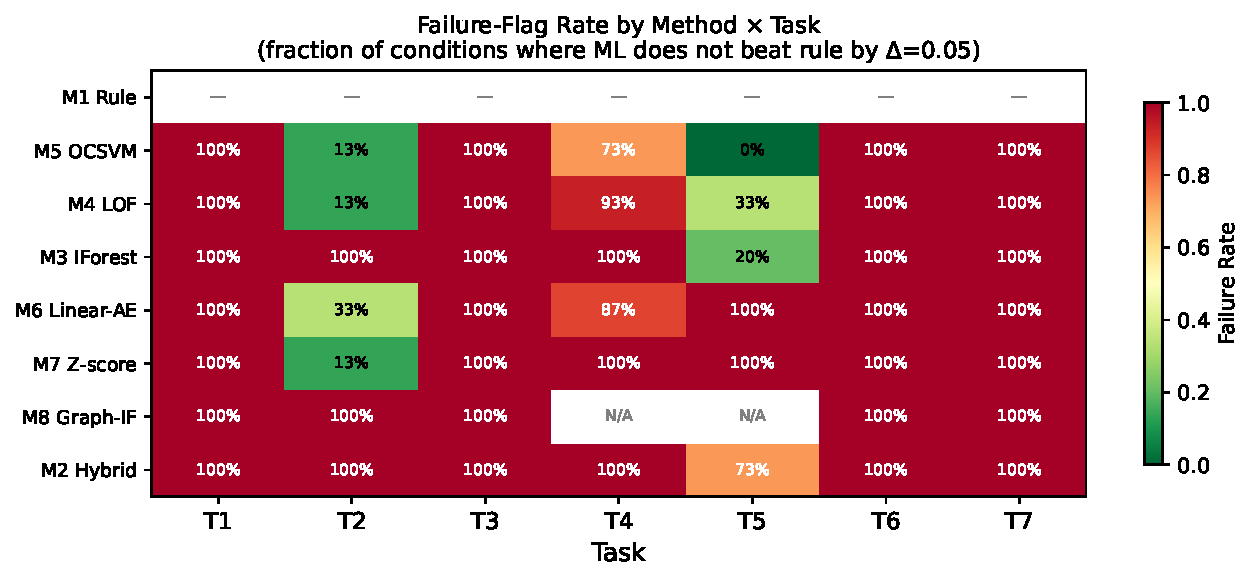
\includegraphics[width=\columnwidth]{figures/fig2_failure_heatmap.pdf}
  \caption{Failure-flag rate heatmap (method $\times$ task). Red cells indicate
    flagged configurations, ML fails to improve on the rule baseline by the
    pre-registered $\Delta$=0.05 threshold (Eq.~\eqref{eq:failure}) in
    $\geq$2/3 seeds; white cells (M8, T4-T5) are not applicable.\\
    \textit{Alt text:} Heatmap of failure-flag rate for 8 methods (rows M1-M8)
    against 7 tasks (columns T1-T7), where each cell shows the percentage of 5
    conditions flagged. Most cells are red at 100\%; green 0\% cells appear where
    ML adds value (for example M5 OCSVM at T2 and T5), and M8 Graph-IF is marked
    N/A for T4 and T5.}
  \label{fig:failure_heatmap}
\end{figure}

\begin{figure}[t]
  \centering
  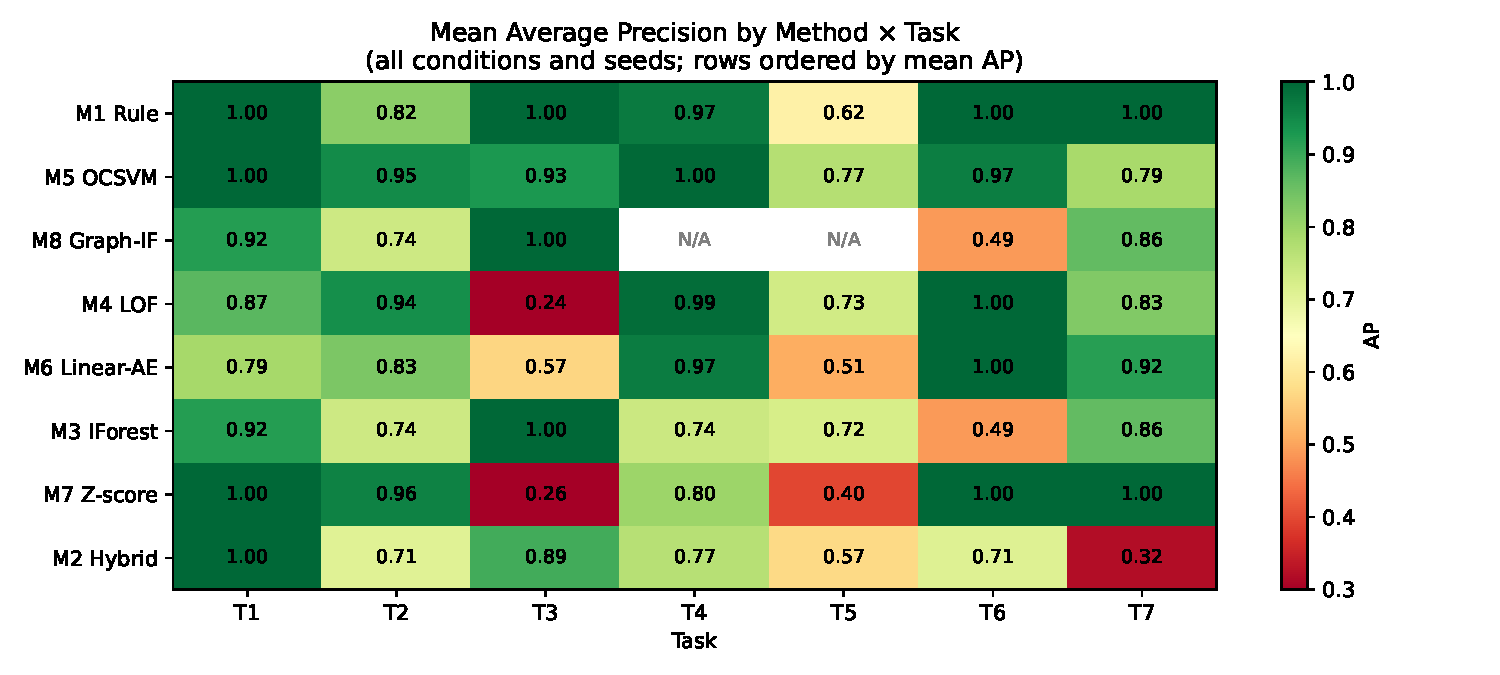
\includegraphics[width=\columnwidth]{figures/fig1_ap_heatmap.pdf}
  \caption{Condition-averaged AP heatmap (method $\times$ task). Higher values
    indicate better anomaly ranking. Rows are ordered by mean AP across all
    runs; M1 (rule baseline) anchors the top row.\\
    \textit{Alt text:} Heatmap of mean average precision for 8 methods (rows
    M1-M8) against 7 tasks (columns T1-T7), with values from about 0.24 to 1.00
    shaded red (low) to green (high). The M1 rule baseline row is highest overall;
    notable low cells include M4 LOF and M7 Z-score at T3, and M8 Graph-IF is N/A
    for T4 and T5.}
  \label{fig:ap_heatmap}
\end{figure}

\begin{figure*}[t]
  \centering
  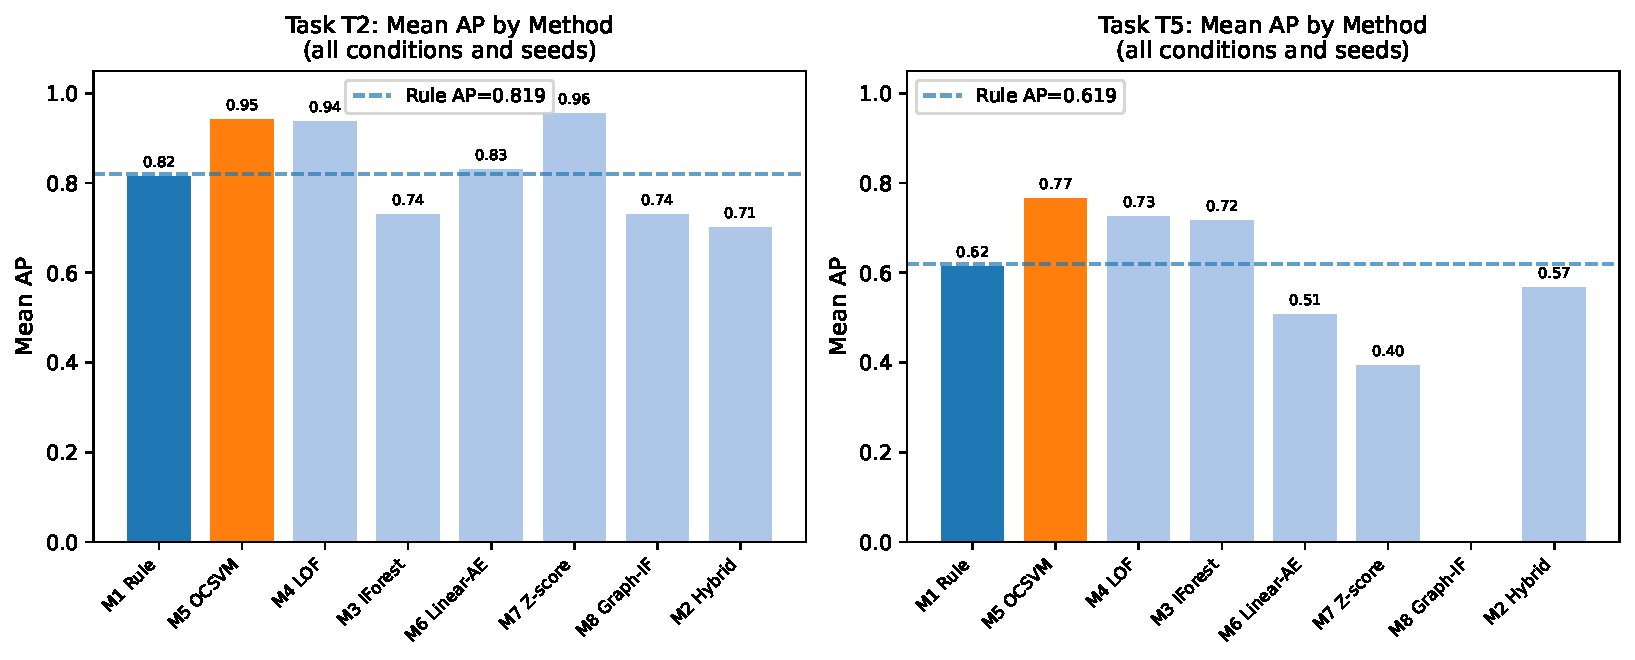
\includegraphics[width=\textwidth]{figures/fig4_t2_t5_ml_gain.pdf}
  \caption{AP by method for T2 (group membership drift) and T5
    (patch-vulnerability hygiene), averaged over all conditions and seeds, the
    two tasks where ML consistently adds value over the rule baseline.\\
    \textit{Alt text:} Two bar charts of mean average precision by method. For
    task T2 several methods exceed the dashed rule baseline of 0.819, led by
    M7 Z-score (0.96) and M5 OCSVM (0.95). For task T5 only M5 OCSVM (0.77) and
    M4 LOF (0.73) clearly beat the rule baseline of 0.619, while M7 Z-score (0.40)
    is the worst.}
  \label{fig:ml_gain}
\end{figure*}

\begin{figure*}[t]
  \centering
  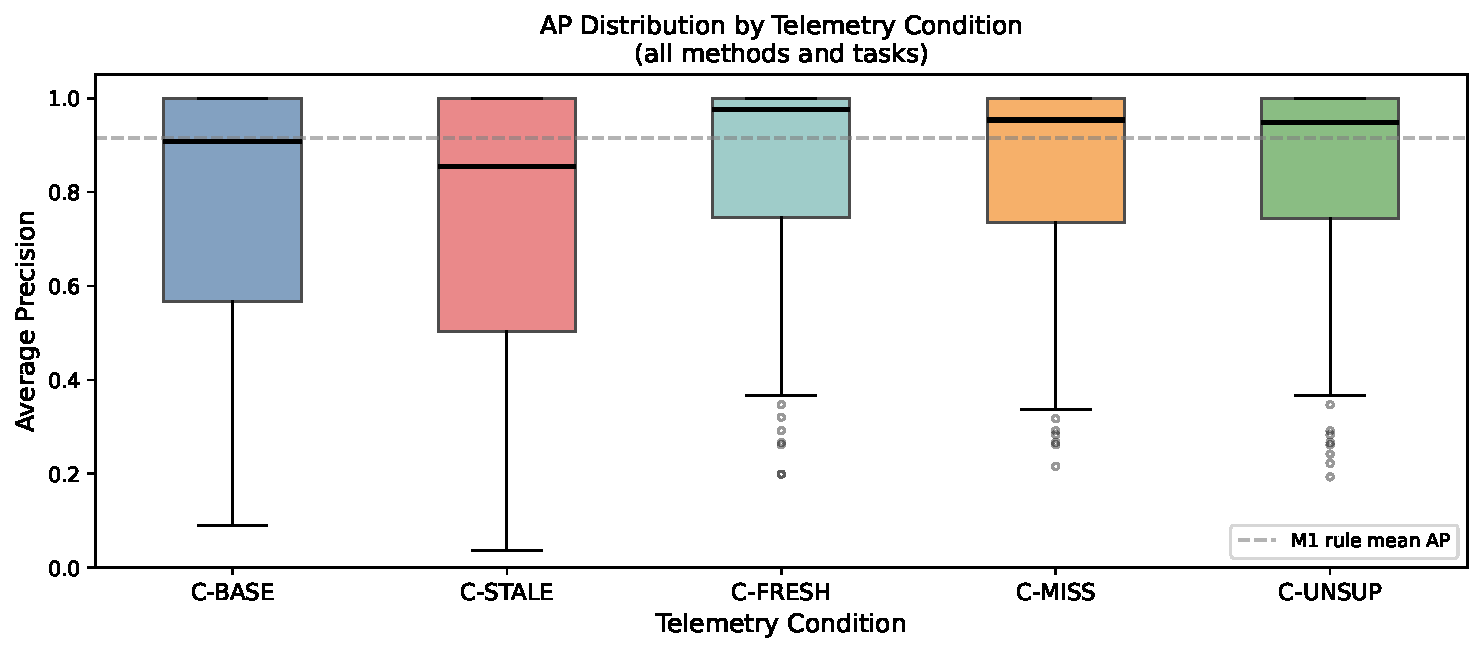
\includegraphics[width=\textwidth]{figures/fig3_ap_by_condition.pdf}
  \caption{AP distribution by telemetry condition (all tasks and methods). C-STALE
    has the lowest mean AP; C-FRESH has the highest.\\
    \textit{Alt text:} Box plots of average precision across five telemetry
    conditions (C-BASE, C-STALE, C-FRESH, C-MISS, C-UNSUP) over all methods and
    tasks. C-STALE shows the lowest and most spread-out distribution, while
    C-FRESH, C-MISS, and C-UNSUP have higher, tighter medians near the dashed
    M1 rule mean AP line, with several low outliers below 0.4.}
  \label{fig:ap_condition}
\end{figure*}

% Section: Discussion
% Source: paper_draft_v0.1.md § 6. Discussion
% [VERIFY ACM TEMPLATE BEFORE SUBMISSION]

\section{Discussion}
\label{sec:discussion}

\subsection{Interpretation of the Negative-Result Finding}

The 86.2\% failure rate is not a finding against ML in security operations broadly.
It is a finding about the relative performance of unsupervised ML versus structured
rule baselines on \emph{synthetic, structured, class-imbalanced tabular anomaly
detection} in the specific domain of cyber-hygiene telemetry.

The synthetic benchmark is, by design, favorable to rule-based methods: anomaly
injection creates features that are directly correlated with the anomaly class in
ways that rule thresholds exploit cleanly. In operational environments, data is
noisier, labels are unavailable, and the feature space is more complex.
\hygienebench reports this limitation explicitly in the dataset card and generator
documentation.

The appropriate takeaway is: for \hygienebench v0.1, ML adds consistent value over
rule baselines specifically on T2 (group membership drift) and T5
(patch/vulnerability hygiene). These tasks involve multi-signal combinations that
benefit from learned representations. Future work should test whether this advantage
persists under increased population-level noise and label sparsity.

\subsection{Limitations}

\paragraph{Synthetic data.}
All telemetry is synthetic. Structural priors are approximate (DBIR 2026 for patch
lag; NVD for CVE severity; CISA BOD 23-01 for freshness cadence). AD group-size
distributions lack a peer-reviewed source and are modeled under disclosed
assumptions. Detection performance on real operational data will differ from
benchmark results.

\paragraph{Approximations in M6 and M8.}
M6 is implemented as PCA-based linear reconstruction error (not a neural
autoencoder) and M8 as networkx graph features + Isolation Forest (not
DOMINANT-style deep graph autoencoder~\cite{ding2019dominant}). These are disclosed
approximations; results may change with full implementations.

\paragraph{Small population scale.}
Medium scale ($n$=1,000 users) limits the statistical power of the evaluation. The
population is smaller than most public-sector environments, which may affect the
generalizability of the class imbalance findings.

\paragraph{Feature engineering as a design choice.}
The task feature extractors (T1--T7) encode domain knowledge about which features
matter. Methods that exploit these features more effectively will appear better. A
fully unsupervised method that discovers relevant features from raw tables is not
evaluated.

\paragraph{Fixed $k$ values.}
P@$k$ is sensitive to the choice of $k$. \hygienebench uses operationally motivated
$k$ values (daily/weekly SOC review budgets) rather than tuning $k$ to maximize
method performance. This is a deliberate design choice but limits comparison to
benchmarks with different $k$ conventions.

\paragraph{No calibration.}
Anomaly scores are not calibrated to probabilities. Calibration is the primary
research question of a separate line of work and is excluded from \hygienebench by
design.

\subsection{Relationship to Prior Work}

\hygienebench is designed to complement, not replace, existing benchmarks. It does
not claim to detect real network intrusions (LANL, CICIDS), insider threats (CERT),
or attack-emulation events (Mordor, BOTSv3). It is the first benchmark, to our
knowledge, that jointly covers Active Directory identity hygiene state, endpoint
patch posture, vulnerability exposure, and telemetry freshness under controlled
conditions with an openly released, reproducible synthetic generator.

% Section: Conclusion
% Source: paper_draft_v0.1.md § 7. Conclusion
% [VERIFY ACM TEMPLATE BEFORE SUBMISSION]

\section{Conclusion}
\label{sec:conclusion}

We introduced \hygienebench, a reproducible synthetic benchmark for cyber-hygiene
anomaly detection, covering seven tasks and twelve anomaly classes across eleven
entity/event tables. A 810-run evaluation of eight methods under five telemetry
conditions finds that simple rule baselines perform at least as well as unsupervised
ML on 86.2\% of (condition, task, method) configurations. ML adds meaningful value
on two of seven tasks---group membership drift (T2, $+$0.185 AP) and
patch/vulnerability hygiene (T5, $+$0.210 AP)---while rule baselines dominate on
tasks with strong single-feature discriminators. Telemetry staleness (C-STALE)
consistently degrades detection performance. These findings motivate honest,
task-stratified evaluation of anomaly detection methods and explicit negative-result
reporting in security benchmark papers.

\hygienebench v0.1, including the synthetic generator, frozen datasets, and
evaluation harness, is openly available at:
\url{https://github.com/Harshavardhanmalla-Labs/research-papers/tree/main/paper3} ---
Zenodo DOI to be finalized at camera-ready submission.
% [NOTE: add Zenodo DOI at camera-ready]


\section*{Data Availability Statement}
The data and code that support the findings of this study are openly available in the research-papers repository at \url{https://github.com/Harshavardhanmalla-Labs/research-papers/tree/main/paper3}. The manuscript sources, figures, analysis code, and frozen result tables are included and regenerate every reported number deterministically from the fixed seeds.

\section*{Disclosure Statement}
No potential conflict of interest was reported by the author.

\section*{Funding}
No funding was received.


% Generated by IEEEtran.bst, version: 1.14 (2015/08/26)
\begin{thebibliography}{10}
\providecommand{\url}[1]{#1}
\csname url@samestyle\endcsname
\providecommand{\newblock}{\relax}
\providecommand{\bibinfo}[2]{#2}
\providecommand{\BIBentrySTDinterwordspacing}{\spaceskip=0pt\relax}
\providecommand{\BIBentryALTinterwordstretchfactor}{4}
\providecommand{\BIBentryALTinterwordspacing}{\spaceskip=\fontdimen2\font plus
\BIBentryALTinterwordstretchfactor\fontdimen3\font minus
  \fontdimen4\font\relax}
\providecommand{\BIBforeignlanguage}[2]{{%
\expandafter\ifx\csname l@#1\endcsname\relax
\typeout{** WARNING: IEEEtran.bst: No hyphenation pattern has been}%
\typeout{** loaded for the language `#1'. Using the pattern for}%
\typeout{** the default language instead.}%
\else
\language=\csname l@#1\endcsname
\fi
#2}}
\providecommand{\BIBdecl}{\relax}
\BIBdecl

\bibitem{verizon_dbir_2026}
{Verizon}, ``{2026 Data Breach Investigations Report},'' Verizon Business,
  2026, \url{https://www.verizon.com/business/resources/reports/dbir/}.

\bibitem{cisa_bod2301_2022}
{CISA}, ``{Binding Operational Directive 23-01: Improving Asset Visibility and
  Vulnerability Detection on Federal Networks},'' Cybersecurity and
  Infrastructure Security Agency, Tech. Rep., Oct. 2022,
  \url{https://www.cisa.gov/binding-operational-directive-23-01}.

\bibitem{nist_sp80040_2022}
{NIST}, ``{SP 800-40 Rev. 4: Guide to Enterprise Patch Management Planning},''
  National Institute of Standards and Technology, Tech. Rep., Apr. 2022,
  \url{https://csrc.nist.gov/publications/detail/sp/800-40/rev-4/final}.

\bibitem{kent2015lanl}
A.~D. Kent, ``{Comprehensive, Multi-Source Cyber-Security Events},'' Los Alamos
  National Laboratory, Tech. Rep., 2015, doi:10.2172/1259877.

\bibitem{glasser2013cert}
J.~Glasser and B.~Lindauer, ``{Bridging the Gap: A Pragmatic Approach to
  Generating Insider Threat Data},'' in \emph{Proceedings of the IEEE Security
  and Privacy Workshops (SPW)}.\hskip 1em plus 0.5em minus 0.4em\relax San
  Francisco, CA, USA: IEEE, 2013, pp. 98-104.

\bibitem{sharafaldin2018cicids}
I.~Sharafaldin, A.~H. Lashkari, and A.~A. Ghorbani, ``{Toward Generating a New
  Intrusion Detection Dataset and Intrusion Traffic Characterization},'' in
  \emph{Proceedings of the 4th International Conference on Information Systems
  Security and Privacy (ICISSP)}.\hskip 1em plus 0.5em minus 0.4em\relax
  Funchal, Madeira, Portugal: SciTePress, 2018, pp. 108-116.

\bibitem{rodriguez2019mordor}
R.~M. Rodriguez, ``{Mordor: Pre-Recorded Security Events},'' GitHub repository,
  2019, \url{https://github.com/OTRF/Security-Datasets}.

\bibitem{darpa_tc_2018}
{DARPA Information Innovation Office (I2O)}, ``{Transparent Computing
  Engagement 3 (TC-E3) Data Release},'' GitHub repository, Aug. 2018,
  \url{https://github.com/darpa-i2o/Transparent-Computing}.

\bibitem{splunk_botsv3}
{Splunk}, ``{Boss of the SOC (BOTS) v3 Dataset},'' GitHub repository, 2018,
  \url{https://github.com/splunk/botsv3}.

\bibitem{ding2019dominant}
K.~Ding, J.~Li, R.~Bhanushali, and H.~Liu, ``{Deep Anomaly Detection on
  Attributed Networks},'' in \emph{Proceedings of the 2019 SIAM International
  Conference on Data Mining (SDM)}.\hskip 1em plus 0.5em minus 0.4em\relax
  Calgary, AB, Canada: SIAM, 2019, pp. 594-602.

\bibitem{liu2024pygod}
K.~Liu, Y.~Dou, X.~Ding, X.~Hu \emph{et~al.}, ``{PyGOD: A Python Library for
  Graph Outlier Detection},'' \emph{Journal of Machine Learning Research},
  vol.~25, no. 141, pp. 1-9, 2024,
  \url{https://www.jmlr.org/papers/v25/23-0963.html}.

\bibitem{creech2013kdd}
G.~Creech and J.~Hu, ``{Generation of a New IDS Test Dataset: Time to Retire
  the KDD Collection},'' in \emph{2013 IEEE Wireless Communications and
  Networking Conference (WCNC)}.\hskip 1em plus 0.5em minus 0.4em\relax
  Shanghai, China: IEEE, 2013, pp. 4487-4492.

\bibitem{sculley2018winners}
D.~Sculley, J.~Snoek, A.~Wiltschko, and A.~Rahimi, ``{Winner's Curse? On Pace,
  Progress, and Empirical Rigor},'' in \emph{Proceedings of the 6th
  International Conference on Learning Representations (ICLR), Workshop
  Track}.\hskip 1em plus 0.5em minus 0.4em\relax Vancouver, BC, Canada:
  OpenReview.net, 2018, pp. 1-4.

\end{thebibliography}


\end{document}
